\documentclass[9pt]{amsart}
\usepackage{amsmath}
\usepackage{amssymb}
\usepackage[parfill]{parskip}
\usepackage{graphicx}
\graphicspath{{../img/}}

\begin{document}
    \newcommand{\me}{
        \author{Abhay Shankar K: cs21btech11001}
        \maketitle
    }
    \title{XV6 assignment report}
    \me

    \section{Overview}

    We have made a single modification to the xv6 code, which writes to the terminal each time the \texttt{log\_write()} function is called. This function may be called from the following functions: 
    \begin{itemize}
        \item \texttt{bzero}: Erases the contents of a block.
        \item \texttt{balloc}: Allocates a disk block to a file.
        \item \texttt{bfree}: Frees a disk block.
        \item \texttt{ialloc}: Allocates an inode when a file is created.
        \item \texttt{iupdate}: Updates the contents of an inode - very frequent.
        \item \texttt{bmap}: Not used.
        \item \texttt{writei}: Writes to a disk block - very frequent.
    \end{itemize}

    \section{Single file}
    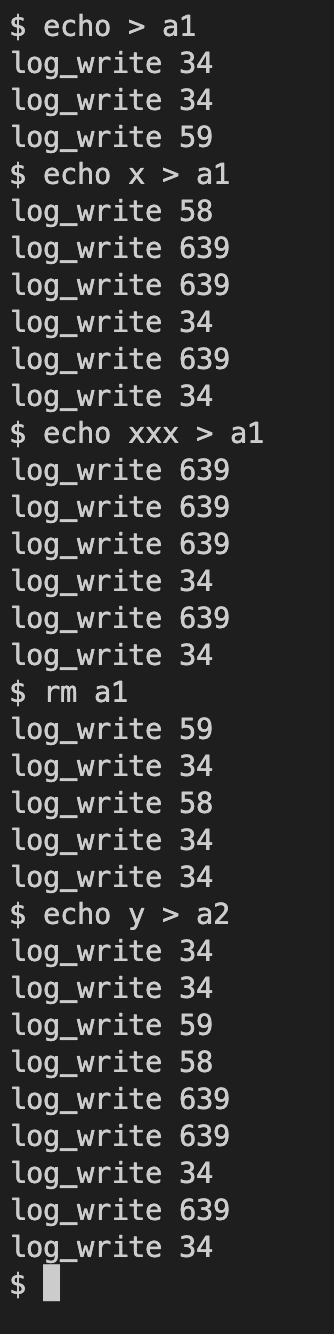
\includegraphics[scale = 0.6]{p1_out.png}
    
    Explanations for each command: 

    \begin{enumerate}
        \item Since a new file is created, the inode (34) is allocated with \texttt{ialloc()} and updated with \texttt{iupdate()}, and the directory (59) is written to with \texttt{writei()}.
        \item The free list - located at block 58 - is updated, and a block (639) is allocated to the new file within \texttt{balloc()}. The contents of block 639 are zeroed using \texttt{bzero()}. 
            
        Then we write data to the block (639 - once per character + 1 for newline) and update the inode (34) each time the size increases - each increment in size results in one \texttt{iupdate()} call and each character written to disk results in one \texttt{writei()} call. 
            
        Here we have two writes, increasing the size from 0 to 2, so there are two logs each for blocks 34 and 639 due to \texttt{iupdate()} and \texttt{writei()} respectively. 
        \item Since the size increases from 2 to 4 (x\(\backslash\)n to xxx\(\backslash\)n) and we write four characters to disk, we have 4 \texttt{writei()} calls for block 639 and 2 \texttt{iupdate()} calls for block 34. 
        \item The rm command unlinks the file, calling \texttt{sys\_unlink()}. It updates the directory (59), removing the entry corresponding to a1 with a \texttt{writei()}. 
        
        It also decrements the number of links to a1 followed by a \texttt{iupdate()} call. 
        
        If the number of links to the file becomes 0, then the file is truncated and the blocks are appended to the free list - \texttt{bfree()} is called for each block within an \texttt{itrunc()} call. 

        Then, the inode is detached from the file by setting the type to 0 - this is followed by a \texttt{iupdate()} call. Then, it is invalidated by setting the valid field to 0.
        
        \item The logs are simply the concatenated logs of 1 and 2.
    \end{enumerate}
    \section{Multiple files}
    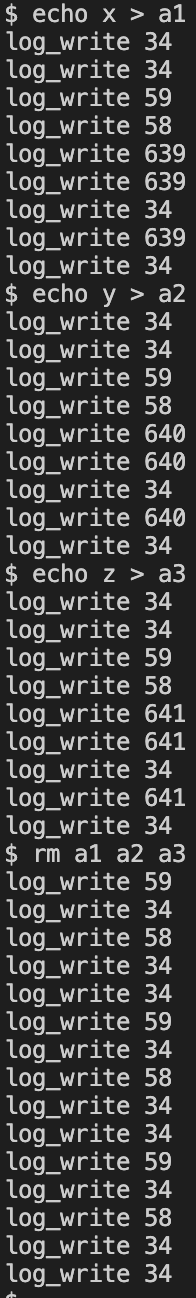
\includegraphics[scale = 0.5]{p2_out.png}

    Explanations:
    \begin{enumerate}
        \item Each of the first three are identical to point 5 in the previous list, except the block number is incremented: 639, 640, 641, as they get popped off the free list.
        
        The mechanism of each command is identical to the previous list.
        \item The removal is also straighforward, and can be viewed as three iterations of point 4 in the previous list. 
    \end{enumerate}
\end{document}I